\chapter{Akku und Ladekonzept}
\fancyfoot[C]{Kern}

%% Übersicht %%%%%%%%%%%%%%%%%%%%%%%%%%%%%%%%%%%%%%%%%%%%%%%
\section{Übersicht}


\subsection{Aufgaben der Energieversorgung}
In den Bereichen der Wirtschaft und der Technik bedeudet der Ausdruck Energieversorgung so viel wie, die Belieferung von Verbrauchern mit Energie. Es gibt unterschiedliche Arten von Energieträgern. Einerseits gibt es leitungsgebundene Energietrieger wie den elektrischen Strom andererseits gibt es auch feste Energieträger wie Kohle oder Holz. In naher Zukunft werden regenerative Energie vermehrt an Bedeutung gewinnen.

Eine stabil Energieversorgung, die mit allen Verbrauchern verbunden ist, wird benötigt, um dem emissionsfreien Sportmotorrad Mobilität zu verleihen. Die Aufgabe der Energieversorgung besteht daher darin, alle Komponenten mit ausreichend Spannung zu versorgen und noch wichtiger, diese Komponenten bei elektrischem Versagen vor Schäden zu schützen. Daher ist die Energieversorgung ein äußerst wichtiger Bestandteil eines solchen Projekts. Im weiteren Verlauf dieses Kapitel wird erklärt, wie die Energieversorgung geplant und in weiterer Folge umgesetzt wurde.

\subsection{Aufgaben des Batteriemanagement}
Wie bereits im Kapitel 2.5 erklärt wurde, bestehen die Aufgaben des Batteriemanagement darin, Kennwerte der Akkumulatoren aufzunehmen und an eine Steuereinheit weiterzuleiten. Weiters ist es auch für den Schutz der Akkumulatoren zuständig und ebenfalls für einen geregelten Ladevorgang.

Ein Bestandteil des Batteriemanagements ist das sogenannte Batteriemanagementsystem (BMS). Das BMS hat die Aufgabe die Akkumulatoren auf ihre Ladung und Entladung zu überwachen und ebenfalls zu regeln. Die Hauptaufgabe des Batteriemanagementsystem besteht jedoch darin, die Restenergie in den Zellen optimal zu nutzen. Um keine Beschädigungen an Zellen zu bekommen, schützt das Batteriemanagementsystem die Batterien vor Tiefenentladung, vor Überspannung, vor zu schneller Ladung (begrenzen des Ladestroms) und ebenfalls vor einem zu hohen Entladestrom. Bei Akkupacks, d.h. Akkumulatoren mit mehreren Zellen, sorgt das Batteriemanagementsystem außerdem für ein sogenanntes Balancing, das sich darin ausdrückt, dass die verschiedenen Batteriezellen gleiche Ladezustände und Entladezustände haben. Das Batteriemanagementsystem liest und verarbeitet alle Daten, die anschließend über ein Bussystem an die Zentralsteuerung weitergegeben werden.

Um die Akkumualtoren beziehungsweise die Akkupacks wieder aufladen zu können, wird ein externes Ladegerät benötigt. Bei Badarf wird dieses Ladegerät mit den Akkumulatoren verbunden um den Ladevorgang in Gang zu setzten.
\newpage

\section{Energieversorgung}
\subsection{Dimensionierung der Akkuzellen}
Es ist besonders wichtig die Daten der Zellen vorher zu beachten um die Dimensionierung gut zu planen und schließlich auch umszusetzten. Um die Energie effizient speicher zu können wurden Lithium-Ionen Akkumulatoren verwendet. Da der Elektromotor mit einer Spannung von 50,4V gespeist werden muss, haben wir uns desswegen auch auf ein solches Versorgungssystem geeinigt. Weiters ist bei Dimensionierung besonders wichtig auf die Lade- und Entladeströme zu achten. Einerseits muss beim Ladestrom nur auf den Strom des Ladegeräts berücksichtigt werden. Andererseits ist es beim Entladestrom etwas komplizierter. Um den Richtwert des Entladestrom einzuhalten, muss der Nennstrom aller Verbraucher in einem System addiert werden.

Der Verbrauch der Steuerelemente setzt sich aus dem verwendeten Raspberry, dem Batteriemanagementsystem und dem Motorcontroller zusammen. Der Raspberry benötigt eine Spannung von 5V und darf eine maximale Leistung von ca. 8W aufweisen. Der Motorcontroller weist eine Nennspannung von 50,4V auf und benötigt eine Leistung von ungefähr 19,5kW. In den folgenden Formel wird der Strom dieser Komponenten berechnet.
\begin{align*}
I_{Raspberry} &= \frac{P_{Raspberry}}{U}=\frac{8 W}{5 V} = 1,6A\\
\end{align*}

\begin{align*}
I_{Motorcontroller} &= \frac{P_{Motorcontroller}}{U}=\frac{19,5 kW}{50,4 V} = 387 A\\
\end{align*}
Natürlich müsst auf der Stromverbrauch des Batteriemanagementsystem mit einberechnet werden. Dieser ist jedoch vernachlässigbar, weil dieser bei wenigen mA liegt.

In der Nachfolgenden Abbildung kann man die Kenndaten einer einzelnen Lithium-Ionen Zelle betrachten. Durch diese Kenndaten setzt sich weitere Dimensionierung des Akkukonzeptes zusammen. 

\begin{figure}[H]
	\begin{center}
		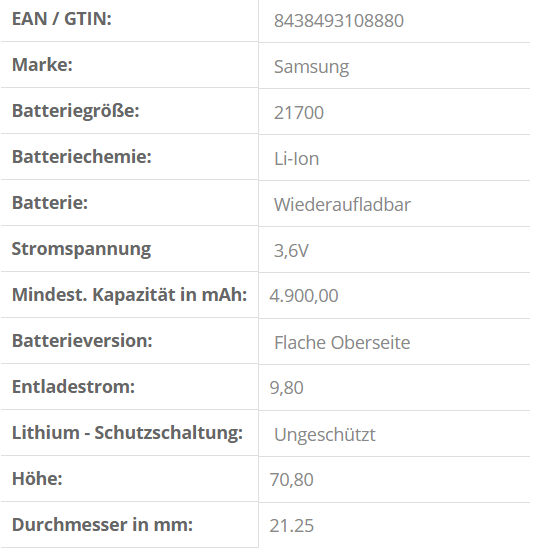
\includegraphics[scale=1.0]{figures/Akku/LithiumIonenZellen.PNG}
		\caption{Eigenschaften und Kennwerte einer Lithium Ionen Zelle}
	\end{center}
\end{figure}

Wie man in der Tabelle erkennen kann, liegt die Spannung einer Lithium Ionen Zelle bei 3,6V. Da jedoch ein Versorgungssystem mit 50,4V notwendig ist müssen die Zellen beziehungsweise die Akkupacks seriell sowie auch parallel verschalten werden. 

Die Nennkapazität einer Zelle beträgt 4900mAh. Um die Kapazität zu erhöhen wurden innerhalb eines Akkupacks 40 einzelne Akkumulatoren parallel verschalten.

\begin{align*}
Q_{Gesamt} &= Q_{Akkupack}= Q_{Zellen} \cdot 40 = 4900~\mathrm{mAh} \cdot 40= 196.000~\mathrm{mAh}\\
\end{align*}

Die Nennkapazität einer Lithium Ionen Zelle beträgt 3,6V. Innerhalb der Akkupacks werden diese 40 Zellen parallel verschalten, was nicht zu einer Erhöhung der Spannung führt. Da wir aber ein Versorgungssystem mit 50,4V benötigen, musst wir die 14 Akkupacks seriell verschalten um die Versorgungsspannung zu erreichen.

\begin{align*}
U_{Gesamt} &= U_{Akkupack} \cdot 14= U_{Zelle} \cdot 14= 3.6~\mathrm{V} \cdot 14 = 50.4~\mathrm{V}\\
\end{align*}

\subsubsection{Zusammenstellung der Batteriezellen}
Die Aufgabe besteht darin, die einzelnen Zellen zu sogenannten Akkupacks zusammenzuschalten. Dafür wurde Abstandshalter verwendet um die Zellen anzuordnen und anschließend mit einem Hiluminband zusammen zu schweißen. 

\begin{figure}[H]
	\begin{center}
		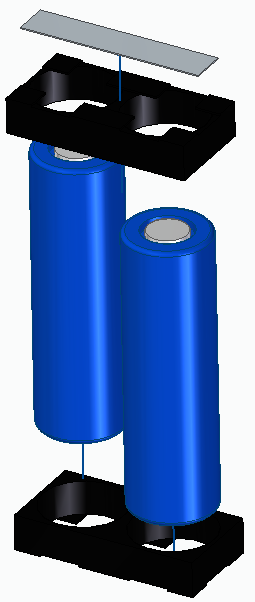
\includegraphics[scale=0.5]{figures/Akku/Explosionsdarstellung2Zellen.PNG}
		\caption{Explosionsdarstellung einer Doppelzelle}
	\end{center}
\end{figure}

Im nächsten Schritt wurden diese Doppelzellen zusammgeschalten, die vereint ein Akkupack ergeben. Die Schwierigkeit dabei war, die Doppelzellen so anzuordnen, dass der Platz in der Schutzbox für die Akkumulatoren möglichst effizient genutzt wird. Jedoch waren wir beim designen der Akkubox realtiv eingeschränkt, da wir darauf achten mussten, diese Boxen auch an unser Motorrad anzubringen. Die Boxen zusammen mit dem Inhalt sind auch extrem schwer. Desswegen war es wichtig, diese Boxen möglicht unten und in der Mitte anzubringen um den Schwerpunkt des emissionsfreien Sportmotorrads nicht drastisch zu verändern.

Wie bereits vorher erwähnt müssen diese Akkupacks geschützt werden. Dies ist notwendig um die Lebenszeit der Akkumulatoren hinauszuzögern und um sie vor äußeren Einflüssen zu schützen. Diese Akkuboxen haben unterschiedliche Formen, da sie an unterschiedlichen Positionen an dem Sportmotorrad angebracht werden. Grundsätzlich haben wir 3 verschiedene Akkuboxen designt und angefertigt.

\textbf{1. Akkubox:}

Die erste Akkubox besteht aus 2 Akkupacks. Das heißt insgesamt beinhaltet sie 80 Zellen.

\begin{figure}[H]
	\begin{center}
		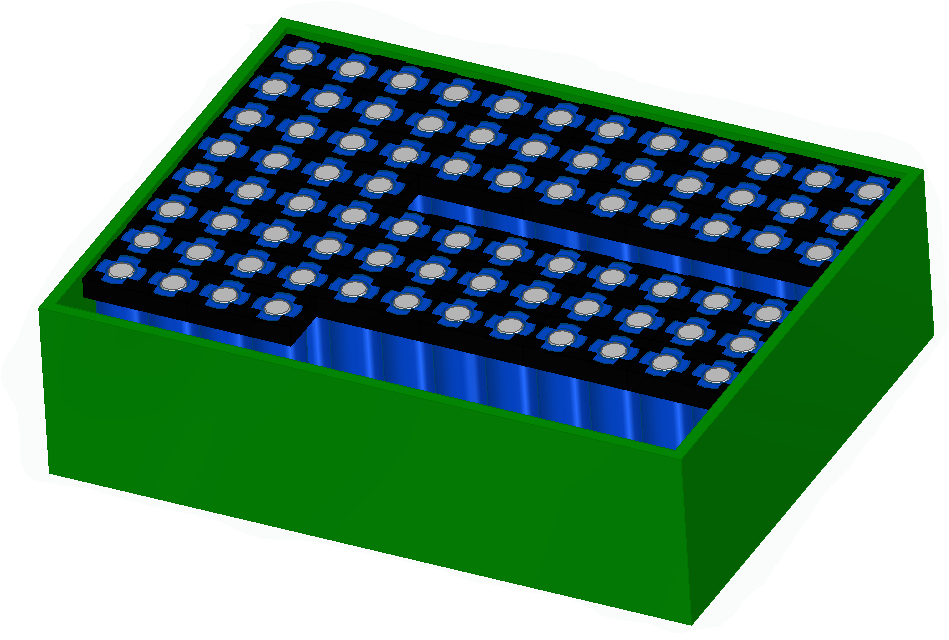
\includegraphics[scale=0.5]{figures/Akku/Akkubox1.PNG}
		\caption{1. Akkubox}
	\end{center}
\end{figure}

\textbf{2. Akkubox:}

Die zweite Akkubox besteht aus insgesamt 6 Akkupacks. Diese Akkubox ist in drei Ebenen aufgeteilt wobei in einer Ebene 2 Akkuboxen Platz finden. Die nächsten beiden Akkuboxen liegen auf der ersten Ebene auf. Schlussendlich befinden sich die letzten 2 der 6 Akkuboxen auf der letzten, der dritten Ebene.

\begin{figure}[H]
	\begin{center}
		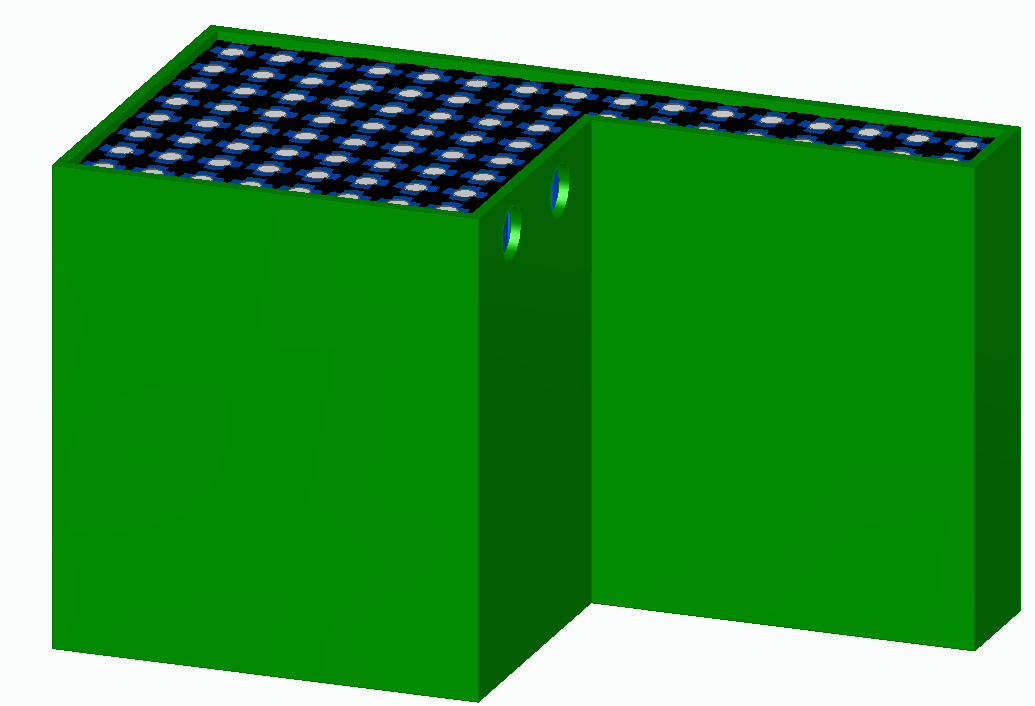
\includegraphics[scale=0.5]{figures/Akku/Box3.PNG}
		\caption{2. Akkubox}
	\end{center}
\end{figure}

\textbf{3. Akkubox:}

Die dritte und somit letzte Akkubox beinhaltet insgesamt 6 Akkupacks. Diese Box wird an der Vorderseite, genauer parallel zu den Stoßdämpfern, angebracht. Es ist wichtig die Box so nahe es geht am Mittelpunkt und möglichst weit in Bodennähe anzubringen, um den Schwerpunkt des Motorrads nicht drastisch zu verändern.

\begin{figure}[H]
	\begin{center}
		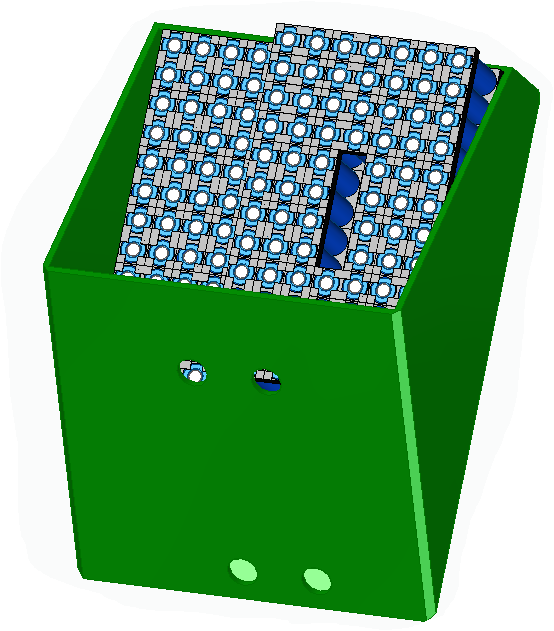
\includegraphics[scale=0.8]{figures/Akku/Akkubox2.PNG}
		\caption{3. Akkubox}
	\end{center}
\end{figure}
\newpage

\subsection{Verschaltung der Batteriezellen}

Bei der Verschaltung der Batteriezellen war es wichtig auf die Kennwerte der Komponenten zu achten. Da unser elektrischer Motor mit einer Spannung von 50,4V versorgt werden muss, haben wir uns daher auch auf ein 50,4V Versorgungssystem geeinigt. Im weiteren Verlauf wurde geplant und schließlich auch umgesetzt wie die Zellen am besten verschaltet werden sollten.

Grundsätzlich gibt es 3 verschiedene Möglichkeiten einzelne Zellen zu verschalten:

\begin{itemize}
\item \textbf{Serienschaltung} 
\item \textbf{Parallelschaltung}
\item \textbf{Kombination aus Serien-und Parallelschaltung}
\end{itemize}

\subsubsection{Serienschaltung}
Das Prinzip der Serienschaltung ist relativ einfach. Der Minuspol der einen Batterie wird einfach mit dem Pluspol der anderen Batterie verbunden. Das hat zur Folge, dass alle Zellen mit dem selben Strom durchflossen werden. Jedoch addieren sich alle Teilspannungen der Zellen zu einer Gesamtspannung. Die Serienschaltung von Batterien wird häufig auch als Hintereinanderschaltung oder Reihenschaltung bezeichnet.

\begin{figure}[H]
	\begin{center}
		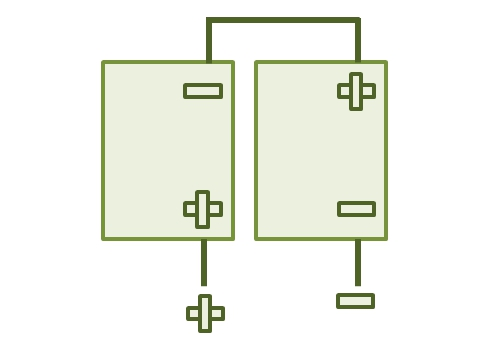
\includegraphics[scale=1.0]{figures/Akku/SerienschaltungzweierBatterien.org.jpg}
		\caption{Serienschaltung beliebig vieler Zellen}
	\end{center}
\end{figure}

Beispiel: Werden zwei Batterien mit jeweils 300Ah (Amperestunden) und 9V (Volt) in Reihe geschaltet, ergibt sich eine Ausgangsspannung von 18V mit einer Kapazität von 300 Ah. \medskip

\textbf{Vorteile und Nachteile:}

Durch die Reihenschaltung wird ermöglicht, höhere Gesmatspannungen zu erzeugen. Ein bedeutender Nachteil ist jedoch, dass die schwächste Zelle die Leistung der gesamten Reihenschaltung beeinflusst. Außerdem kann es vorkommen, dass wenn eine einzelne Batteriezelle defekt ist, die gesamte Batteriereihe ausfällt. Daher ist es notwendig zusätzliche Sicherungen hinzu zu schalten. Im Normalfall können nur Batteriezellen vom gleichen Hersteller, Typ und von der selben Batterietechnik kombiniert und in Serie geschalten werden.
\newpage

\subsubsection{Parallelschaltung}
Das Prinzip der Parallelschatung ist relativ ähnlich zu der Serienschaltung. Der große Unterschied jedoch besteht darin, dass der Minuspol der einen Batterie mit dem Minuspol der anderen Batterie verschaltet wird. Dadurch summieren sich die Ladekapazitäten (Ah) der einzelnen Zellen zu einer gesmaten Ladekapazität. Die Gesamtspannung entspricht jedoch der Spannung einer einzelnen Batterie. 

\begin{figure}[H]
	\begin{center}
		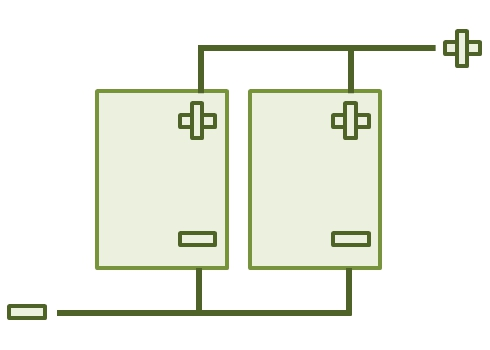
\includegraphics[scale=1.0]{figures/Akku/ParallelschaltungzweierBatterien.org.jpg}
		\caption{Parallelschaltung beliebig vieler Zellen}
	\end{center}
\end{figure}

Beispiel: Werden zwei Batterien mit jeweils 300 Ah und 9V parallel geschaltet, so ergibt sich eine Ausgangsspannung von 9V und eine Gesamtkapazität von 600Ah. \medskip

\textbf{Vorteile und Nachteile:}

Die Parallelschaltung führt dazu, die Leistungsfähigkeit und außerdem die Lebensdauer zu steigern. Jedoch ist die Laderegelung bei einer Parallelschaltung nicht unkompliziert, da jede Zelle unterschiedlich schnell altert und damit einer Fehlerquelle darstellen kann. Deshalb kann es vorteilhaft sein, eine größere Batterie anstatt mehrerer einzelner Zellen zu verwenden. Sollte trotzdem einer Parallelschaltung mehrerer Zellen vorgenommen werden, sollt unbedingt darauf geachtet werden Batterien mit gleicher, Kpapzität, Bauart und Ladezustand einzusetzten. Außerdem ist es von Vorteil möglichst kurze Leitungen einzusetzten, um Spannungsverlust zu verhindern.
\newpage

\subsubsection{Kombination aus Serien- und Parallelschaltung}
Durch eine Kombination aus einer Serien- und Parallelschaltung ermöglicht man eine größeres Flexibilität zur Erreichung einer bestimmten Spannung und auch Leistung. Wie bereits vorher erwähnt erreicht man durch eine Parallelschaltung die benötigte Gesamtkapazität und durch die Serienschaltung die gewünscht Betriebsspannung.

Diese Methode wird in der Praxis am häufigsten eingesetzt und ist auch bei unserem Akkusystem zum Einsatz gekommen.

\textbf{Verschaltung der einzelnen Zellen in den Akkupacks:}

Da wir uns auf ein 50,4V Versorgungssystem geeinigt haben, und jede einzelne Zelle eine Spannung von 3,6V aufweist haben wir jeweils 40 einzelne Lithium Ionen Akkus zusammgeschaltet. Die einzelnen Batterie werden in den Akkupacks parallel verschaltet, da wir so einen deutlich höhere Leistungsfähigkeit erreichen und die Lebensdauer dadurch verlängert wird. 

\begin{figure}[H]
	\begin{center}
		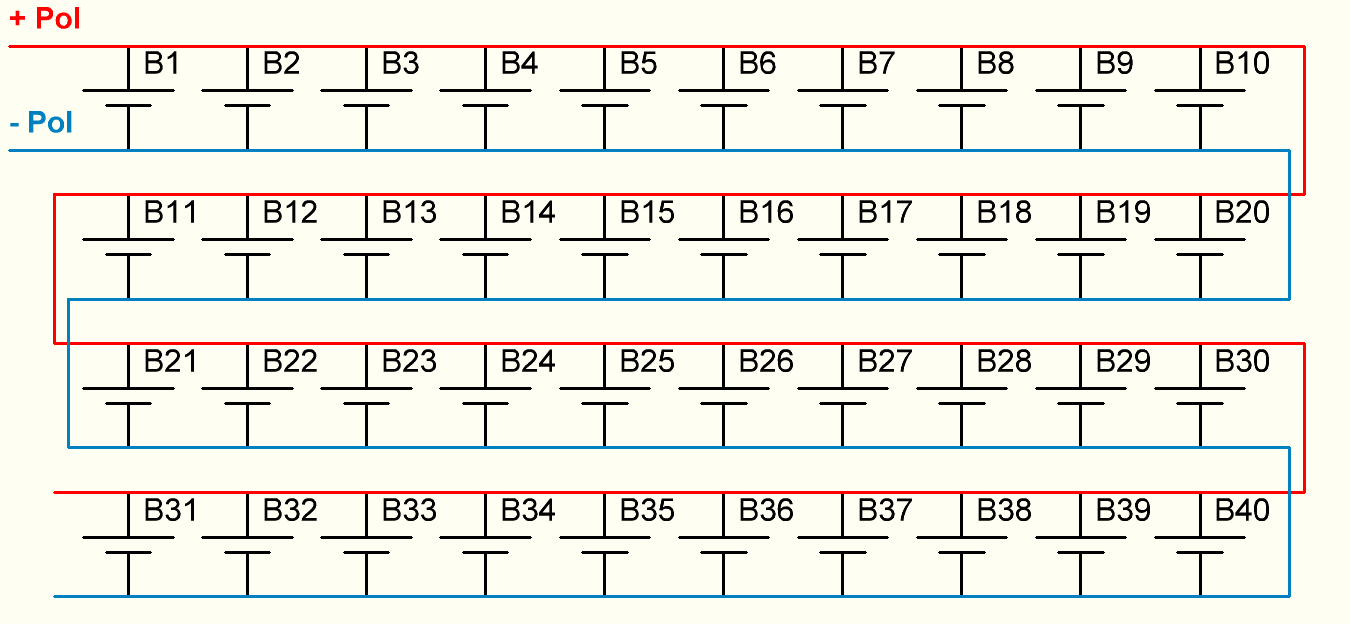
\includegraphics[scale=0.6]{figures/Akku/Anschlussplan 40Zellen.PNG}
		\caption{Verschaltung der einzelnen Zellen innerhalb der Akkupacks}
	\end{center}
\end{figure}
\newpage

\textbf{Verschaltung der Akkupacks:}

Durch die Parallelschaltung innerhalb der Akkupacks wird jedoch nicht die Spannung erhöht. Wir haben eine Anzahl von 560 einzelnen Lithium Ionen Zellen. Ein Akkupack beinhaltet 40 Zellen was dazu führt, dass wir insgesamt 14 Akkupacks haben. Diese 14 Akkupacks werden seriell verschalten um die Spannung von 3,6V auf die gewünschten 50,4V zu vergrößern.

Die seperaten Zellen werden mithilfe eines Hiluminband Punktgeschweißt um so eine Verbindung zwischen den Zellen herzustellen.
Wichtig ist darauf zu achten, dass das Hiluminband nur bis zu einer Stromstärke von 30A zulässig ist. Da wir jedoch weitaus höhere Ströme zu erwarten haben, muss wir dieses Hiluminband verstärkern. Dies erfolt über eine Metallplatte die jeweils an der Oberseite sowie auch an der Unterseite angebracht wird. Dadurch wird die Schweißverbindung gestärkt und in weiterer Folge werden keine Fehler auftreten. 

\begin{align*}
U_{Gesamt} &= U_{Akkupack} \cdot 14= U_{Zelle} \cdot 14= 3.6~\mathrm{V} \cdot 14 = 50.4~\mathrm{V}\\
\end{align*}

Aus Darstellungsgründen wurden die Akkupacks 4 - 13 durch das  Akkupack ... ersetzt.

\begin{figure}[H]
	\begin{center}
		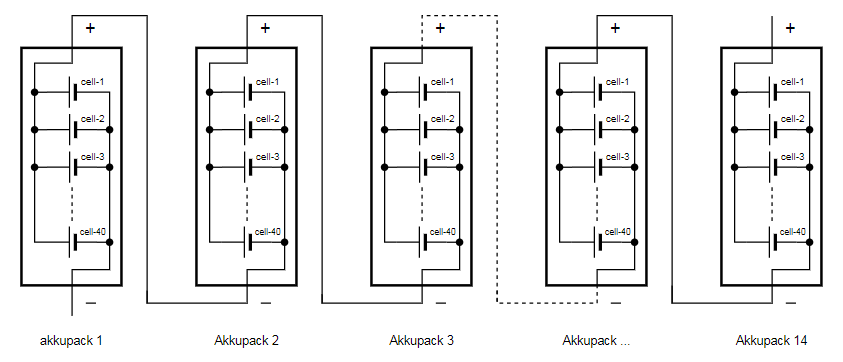
\includegraphics[scale=0.9]{figures/Akku/VerschaltungderAkkupacks.PNG}
		\caption{Verschaltung der Akkupacks}
	\end{center}
\end{figure}
\newpage
\subsubsection{Geschätzt Betriebszeit des Akkumulators}

In diesem Abschnitt wurden alle relevanten Daten gesammelt, um schließlich eine Näherung für die Laufzeit des Akkumulators durchzuführen. Diese Daten wurden bereits im Kapitel Dimensionierung teilwiese berechnet.

Im ersten Schritt wird die Energie, die der Akkumulator aufnehmen kann berechnet.

\begin{align*}
W_{Akkumulator} &= U_{Gesamt} \cdot Q_{Gesamt} = 50.4~\mathrm{V} \cdot 196.000~\mathrm{mAh} = 9880~\mathrm{Wh}\\
\end{align*}

Als nächstes wird die Leistung berechnet. Da sich das Motorrad jedoch nicht immer mit voller Geschwindigkeit fortbewegen wird, haben wir eine Auslastung von 75 Prozent angenommen und eine realistische Akkulaufzeit zu berechnen.

\begin{align*}
P_{Gesamt} &= P_{Motorcontroller} \cdot P_{Raspberry} = 19.5~\mathrm{kW} \cdot 8~\mathrm{W} = 19.508~\mathrm{kW}\\
\end{align*}

Wie bereits vorher erwähnt müssen von dieser berechneten Gesmatleistung 25 Prozent abgezogen werden.

\begin{align*}
P_{Gesamt,real} &= P_{Gesamt} \cdot 75% = 19.508~\mathrm{kW} \cdot 0.75 = 14.63~\mathrm{kW}\\
\end{align*}

Schlussendlich kann die ungefähre Laufzeit des emissionsfreien Sportmotorads berechnet werden.

\begin{align*}
t_{Laufzeit} &= \frac{W_{Akkumualtor}}{P_{Gesamt,real}} = \frac{9880~\mathrm{Wh}}{14.63~\mathrm{kW}} = 0,68~\mathrm{h} = 41~\mathrm{min}\\
\end{align*}

Die geschätzte durch eine Näherung berechnet Laufzeit des Akkumulator, beträgt in etwa 41min.

\subsection{Allgemeine Übersicht der Elektroinstallation}
\newpage
%% Batteriemanagement %%%%%%%%%%%%%%%%%%%%%%%%%%%%%%%%%%%%%%%%%
\subsection{Batteriemanagementsystem}
Der zweite Teil, der für ein funktionierendes Akkusystem notwendig ist, ist das Batteriemanagementsystem. Die Aufgabe des BMS ist es die Akkumulatoren zu überwachen und an die aufgenommenen Daten über eine serielle Schnittstelle an die Zentralsteuerung weiterzugeben. 

In unserm Projekt wurde ein 14S 48V 100A Li-ion Daly BMS Battery Management System verwendet. Wie bereits vorher erwähnt beinhaltet unser Akkusystem 560 Zellen. Die Bezeichnung 14s bedeudet, dass das Batteriemanagement insgesamt maximal 14 Zellen überwachen kann. Daher ist es nicht möglich jede Zelle einzeln zu überwachen da so viele Anschlüsse nicht vorhanden sind. Jedes Akkupack beinhaltet 40 Zellen.

\begin{align*}
Akkupacks &= \frac{Zellen_{gesamt}}{Zellen_{Akkupack}} = \frac{560~\mathrm{Zellen}}{40~\mathrm{Zellen}} = 14~\mathrm{Akkupacks}\\
\end{align*}

\begin{figure}[H]
	\begin{center}
		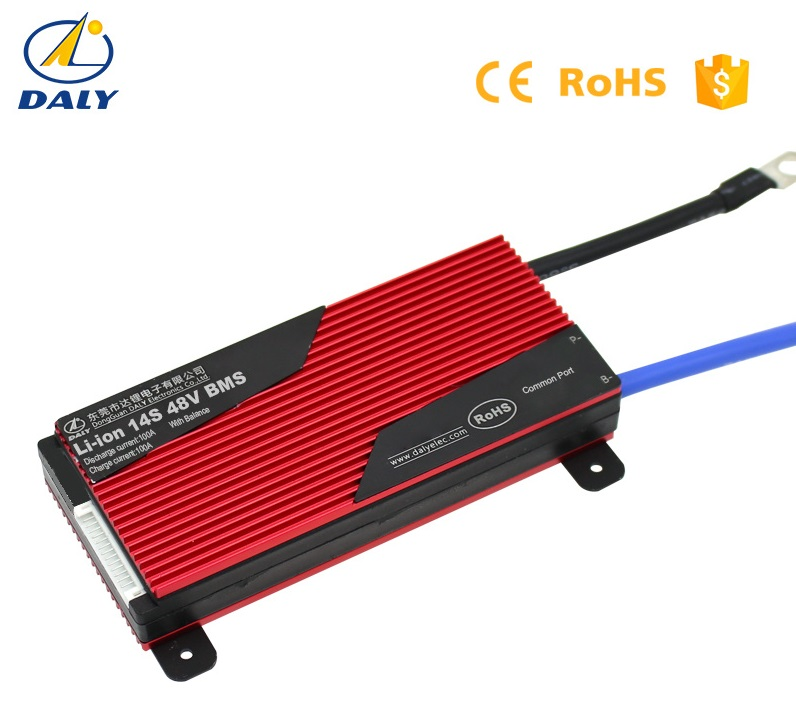
\includegraphics[scale=0.9]{figures/Akku/Daly Batteriemanagementsystem.jpg}
		\caption{Caly Batteriemanagementsystem}
	\end{center}
\end{figure}

\subsubsection{Funktionen des Batteriemanagementsystems}

Unter dem Begriff Batteriemanagementsystem versteht man die Überwachung und Regelung von Akkumulatoren beim Laden und ebenfalls Entladen. Ein BMS ist nichts anderes als eine elktronische Regelschaltung. Zu den häufigsten Batteriekennwerten gehören die Erkennung des Batterietyps, die Batteriespannung, die Spannung sowie die Temperatur einzelner Akkumulatoren oder gesamter Akkupacks, die Akkukapazität, der Ladezustand, die Restbetriebszeit, die Stromentnahme und einige Kennwerte mehr. Die Aufgabe des Batteriemanagementsystems besteht also darin, sichzugehen, dass die Energie in einer Zellen effizient genutzt wird. Um Beschädigungen von Akkus zu vermeiden, haben die Akkus einen Tiefentladungsschutz, einen Überspannungsschutz und außerdem schützt das BMS auch vor zu schneller Ladung und ebenfalls vor einem zu hohen Entladestrom. Oft ist es der Fall, dass in einem Projekt mehrere einzelne Akkus oder sogar Akkupacks zum Einsatz kommen. In einem solchen Fall sorgt das Batteriemanagementsystem für ein sogenanntes Balancing. Das Battery-Balancing sorgt dafür, dass die Akkupacks oder einzelne Zellen gleiche Ladezustände und Entladezustände haben. 

In den folgenden Unterpunkten werden die Funktionen des Batteriemanagementsystems genauer erklärt.

\textbf{Balancing:}
Grundsätzlich wurde das Battery-Balancing bereits im ........................................................................................
\textbf{Akkupacks:}

Muss noch zitiert werden: Cluster oder Akkupacks bestehen zur Erhöhung der Nennspannung in der Regel aus mehreren in Reihe geschalteten Einzelzellen oder Zellblöcken. Fertigungs- und alterungsbedingt gibt es hierbei Schwankungen in der Kapazität, im Innenwiderstand und weiteren Parametern dieser Zellen. Die schwächste Zelle ist dabei bestimmend, wie viel geladen oder entladen werden darf. Im praktischen Einsatz von mehrzelligen in Reihe verschalteten Akkus führt dieser Umstand dazu, dass die Zellen in Reihe unterschiedlich geladen und entladen werden.

Es kommt dann im Verbund zu kritischer Tiefentladung oder bei der Ladung zu einer Überladung und Überschreiten der Ladeschlussspannung einzelner Zellen. Je nach Akkutyp kann es dabei zu einer irreversiblen Schädigung einzelner Zellen kommen. Die Folge: das gesamte Akkupack verliert an Kapazität. (Ende des Zitates)
Um das zu verhindern, spielen im Batteriemanagementsystem die Balancer eine wichtige Rolle. Beim Battery-Balancing gibt es zwei verschiedene Arten. 
\begin{itemize}
\item \textbf{Passives Battery-Balancing} \medskip\\
\item \textbf{Aktives Battery-Balancing} \medskip\\
\end{itemize}

\begin{figure}[H]
	\begin{center}
		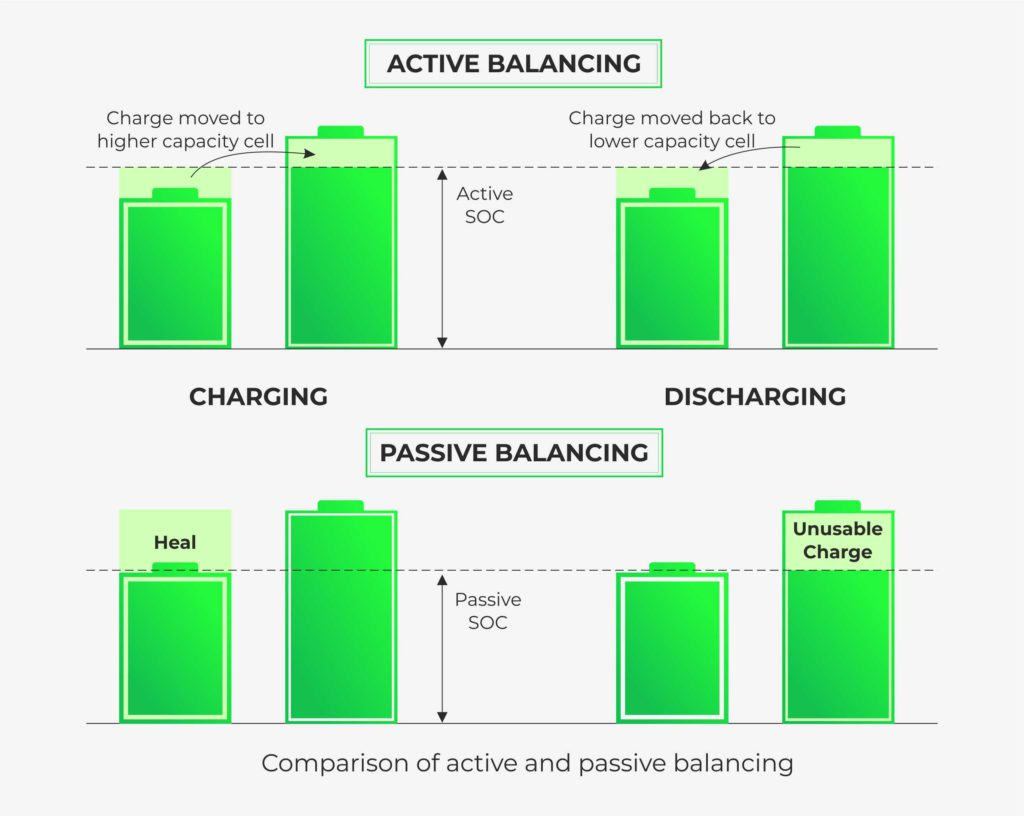
\includegraphics[scale=1.5]{figures/Akku/Vergleichaktivespassives.jpg}
		\caption{Vergleich zwischen Aktiven- und Passiven-Battery Balancing}
	\end{center}
\end{figure}
\newpage

\textbf{Passives Battery-Balancing:}

Eine technische weit verbreitete Methode für das Balancing, ist das Passive Battery-Balancing. Dabei arbeitet es nur im Bereich des Ladeschlusses. Der Ausdruck Ladeschluss bedeutet soviel, dass wenn die Akkumulatoren fast vollständig aufgeladen sind das Balancing zu arbeiten beginnt. Sobald die Zellen die Ladeschlussspannung erreicht haben, wird durch den Balancer ein Widerstand parallel dazugeschalten, um so die Spannung auf die Ladeschlussspannung zu begrenzen. Zellen, welche diese Spannung bereits erreicht haben, werden dann nur noch geringfügig weitergeladen oder teilweise sogar etwas entladen. Die Zellen, die jedoch noch in der Reihenschaltung verschalten sind und die Ladeschlussspannung noch nicht erreicht haben, werden weiterhin mit dem Ladestrom versorgt und somit weitergeladen. Wichtig ist darauf zu achten, dass die Leistung des Parallelwiderstandes auf den Ladstrom angepasst werden muss, da sonst zuviel Energie in Form von Wärme am Widerstand auftreten wird.

\begin{figure}[H]
	\begin{center}
		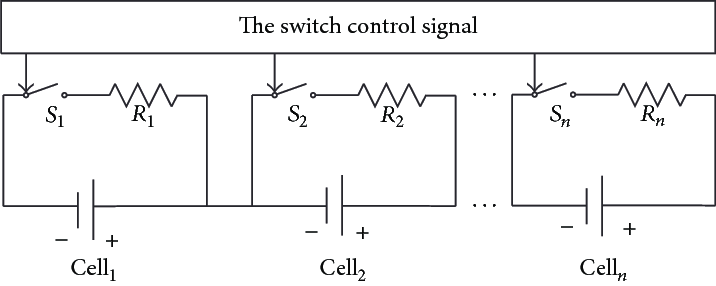
\includegraphics[scale=0.5]{figures/Akku/Passive-cell-balancing.png}
		\caption{Funktionsweise des Passiven Battery-Balancing}
	\end{center}
\end{figure}

\textbf{Vorteile} des Passiven Battery-Balancing:
\begin{itemize}
\item {sehr kostengünsigt} \medskip\\
\item {technisch relativ leicht realisierbar} \medskip\\
\end{itemize}

\textbf{Nachteile} des Passiven Battery-Balancing:
\begin{itemize}
\item {Ladevorgang kann extrem lange dauern, da man warten muss bis die schwächste Zelle den geforderten State of Charge (SOC) erreicht hat} \medskip\\
\item {viel Energie verpufft in Form von Wärme} \medskip\\
\item {Diese Verlustwärme wirkt sich negativ auf die Lebensdauer der Akkumulatoren aus} \medskip\\
\item {nicht unerhebliche Brandgefahr} \medskip\\
\end{itemize}
\newpage

\textbf{Aktives Battery-Balancing:}

Diese Methode des Balancing ist etwas komplexer als beim Passiven Battery-Balancing, jedoch ist sie deutlich effizienter. Bei den aktiven Balancern wird ein Ladungstransfer von Zellen untereinander realisiert. Das bedeutet, dass die Energie der Zellen die bereits ein höher Ladung aufweisen, auf die Akkumulatoren mit niedrigerer Ladung übertragen werden. Beim Aktiven Battery-Balancing werden sogenannte Ladreglungen benötigt. Ladreglungen sind im Prinzip speziell auf eine Anwendung optimierte Schaltregler, die pro Zelle arbeiten und aktiv die Energie übertragen. Dieser Vorgang kann bereits während des Ladeprozesses erfolgen. Standartmäßig wird dieser Vorgang jedoch erst im Bereich des Ladeschlusses aktiv (gleich wie beim Passiven Battery-Balancing). Eine weiterentwickelte Form dieses Systems wird bidirektionalens Balancer-System genannt. Hierbei ist es möglich, dass des Ladungsaustausch sowohl beim Entladen als auch beim Aufladen der Zellen stattfinden kann. Desswegen sind diese bidrektionalen Balancer noch deutlich effizienter. Das Akitve Battery-Balancing wird heutzutage meistens bei größeren Leistungen angewandt, wie zum Beispiel im Bereich der Elektromobilität.

\begin{figure}[H]
	\begin{center}
		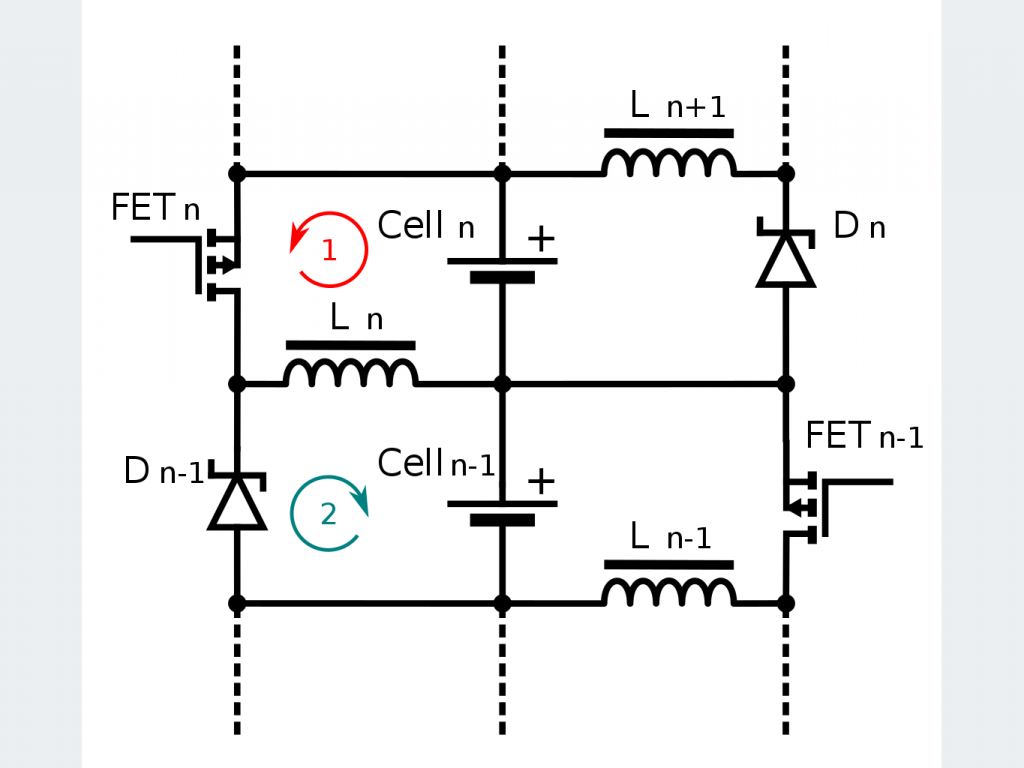
\includegraphics[scale=0.4]{figures/Akku/Aktives Balancing.png}
		\caption{Funktionsweise des Aktiven Battery-Balancing}
	\end{center}
\end{figure}

In der obigen Abbildung kann man die Prinzipschaltung eines aktiven Balancers mit zwei Stufen sehen. Innerhalb von zwei Schaltvorgängen kann dabei die Energie aus der Akkuzelle Cell n über den FET n in die Spule L n übertragen werden (Schleife in rot, 1).
Im zweiten Schaltvorgang (Schleife in blau, 2) wird die Energie in der Spule L n über Diode D n-1 in die Cell n-1 geladen und Cell n-1 aufgeladen.

\textbf{Vorteile} des Aktiven Battery-Balancing:
\begin{itemize}
\item {deutlich höherer Wirkungsgrad als beim passiven Battery-Balancing} \medskip\\
\item {übergeordnete Ladereglung mit intelligenter und lernfähiger Software} \medskip\\
\item {Lebensdauer der Akkumulatoren kann durch die Methode der Ladungsumverteilung deutlich erhöht werden} \medskip\\
\item {überschüssige Energie wird nur zu einem geringen Grad in Wärme umgewandelt} \medskip\\
\item {geringeres Risiko für eine Entflammung} \medskip\\
\end{itemize}

\textbf{Nachteile} des Aktiven Battery-Balancing:
\begin{itemize}
\item {höherer Verschaltungsaufwand, dadurch erhöhte Initialkosten} \medskip\\
\end{itemize}

\subsection{Akkumulatoren}
Um Beschädigungen von Lithium-Ionen-Akkus zu vermeiden haben die Akkus einen Tiefentladungsschutz. Für die Regelung überprüft das Batteriemanagementsystem die Restenergie, State of Health (SoH) und den Ladezustand, State of Charge (SoC). Die Werte werden an einen Prozessor übermittelt auf dem die BMS-Software läuft und der SoC-Algorithmus implementiert ist.


\subsection{Akkumulatoren}
\subsubsection{Lithiumbatterien}
